
\section{Adquisición de datos}
\subsection{Registros de ``Leche''}
En el establo de alimentación y dosificación de concentrado, es donde se realizan las tareas de ordeño para las vacas que aportan a la producción neta de leche. El ordeño y la extracción de la leche se ha realizado de manera manual desde sus inicios, pero cuentan con sistemas de ordeño mecánico desde los últimos años. El pesaje de la leche se realiza en kilogramos y el registro de los datos de producción lechera se ha realizado de manera manual en diarios históricos de producción neta. Un ejemplar de estos diarios puede observarse a continuación en la figura \ref{regleche1png}:

\begin{figure}[H]
	 \begin{center}
	 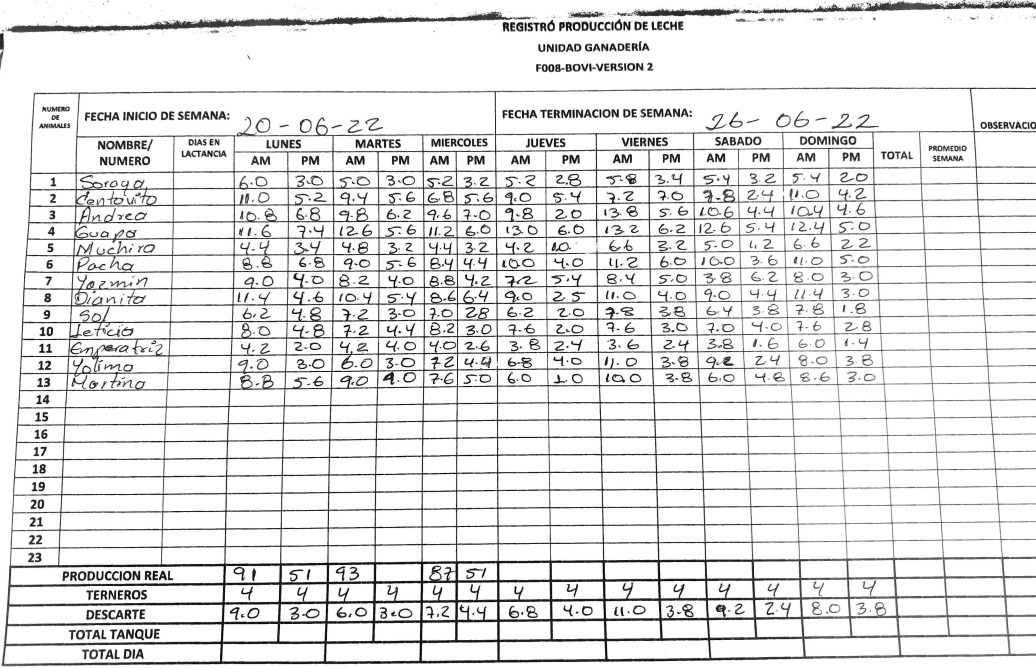
\includegraphics[scale=0.515]{img/regleche1.jpg}
	 \end{center}
	 \caption{Registros manuales de producción lechera en el CA-SENA-POP. \label{regleche1png}}
	\end{figure}
	
Tal y como se puede observar, se lleva un registro diario de cada una de las vacas que se encuentran en etapa de ordeño. Los ordeños se realizan en 2 franjas horarias, en las mañanas, aproximadamente a las 6:00 am, que se realiza el ordeño matutino; y en las tardes, aproximadamente a las 4:00 pm, que se realiza el ordeño vespertino. El registro de los datos se realiza en hojas cuadriculadas donde se puede evidenciar, la producción diaria de cada animal, así como también la producción diaria neta de la unidad de ganadería. Los datos aquí registrados también permiten observar si hay leche que ha sido suministrada a los terneros o si ha sido descartada por sospecha de mastitis, entre otros motivos. \\
	
Aún cuando se lleva un registro manual de los datos, en los últimos 5 años se dio inicio a una migración de datos de manera tecnológica, mediante licencias de software de pago para manejo de producciones ganaderas, entre ellas la licencia del software ``TaurusWebs'' (ver figura \ref{tauruspng}). Sin embargo, esta transición tecnológica no ha sido implementada en su totalidad, por lo que el registro de datos, se realiza de ambas formas en pro de que los datos no se pierdan. Por otra parte, el manejo de datos manual es utilizado para que sirva de material de estudio y aprendizaje en las diferentes actividades y servicios ofrecidos por el SENA, tales como los cursos de formación y capacitación de ganadería.

\begin{figure}[H]
	 \begin{center}
	 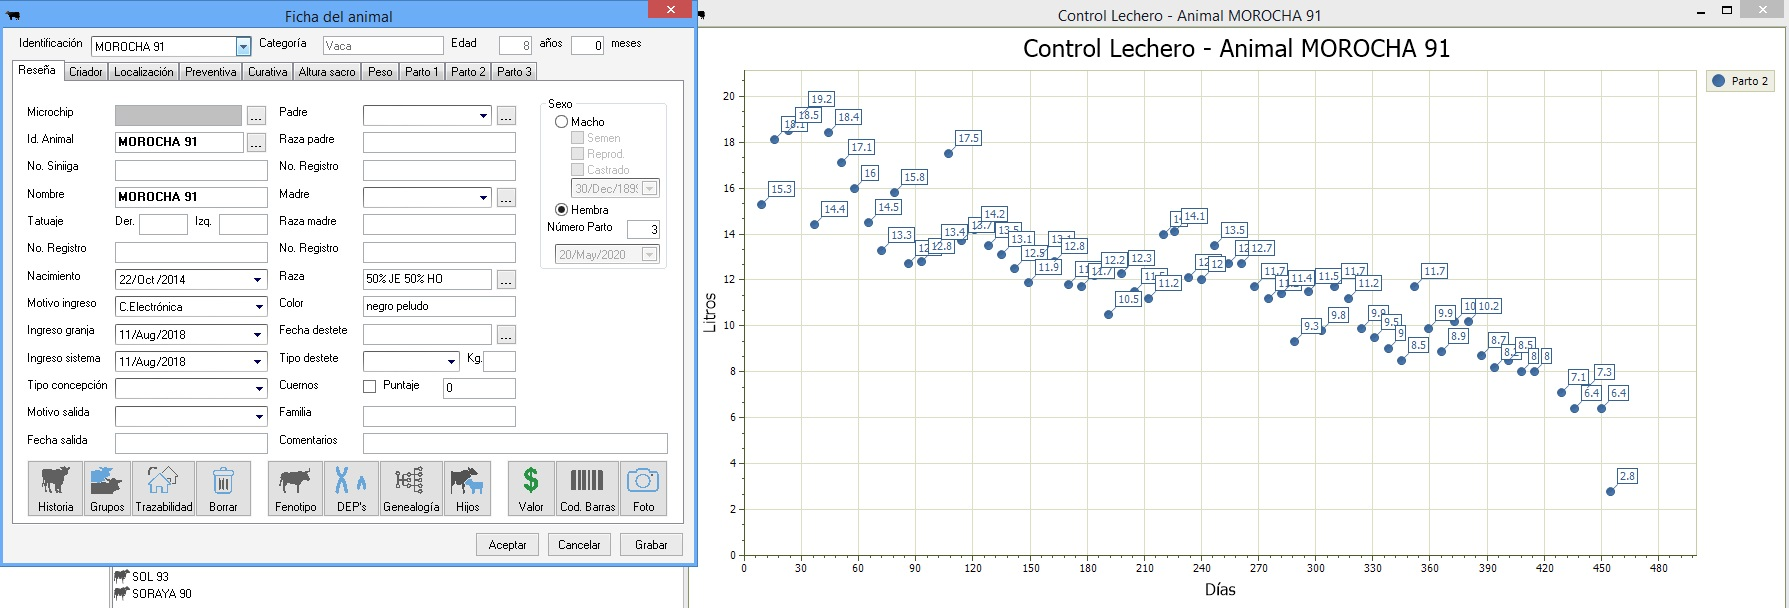
\includegraphics[scale=0.345]{img/ejtaurus.jpg}
	 \end{center}
	 \caption{Registro de datos digital con software TaurusWebs. \label{tauruspng}}
\end{figure}

Una de las ventajas de este software es que alberga una gran variedad de aplicaciones de seguimiento entre las que se pueden mencionar el seguimiento a los registros de leche, registros de peso, registros de antecedentes familiares, trazabilidad, historia, genealogía, entre otros; información que será útil para etapas posteriores en este trabajo.

\subsection{Registros de ``Peso''}

En cuanto a los registros de peso de los animales, El software ``TaurusWebs'' mencionado anteriormente, facilita una hoja de datos donde se pueden almacenar los valores asociados al peso, así como también las fechas en las que fueron realizadas; permitiendo representar dichos datos en gráfica de seguimiento como las que se pueden evidenciar  en la figura \ref{ejpesos}. Estos datos guardados con su fecha de pesaje permiten hacer análisis y algunas observaciones de variabilidad de peso para los distintos partos en los que se agrupan las reses cuyos datos modelan al sistema.

\begin{figure}[H]
	 \begin{center}
	 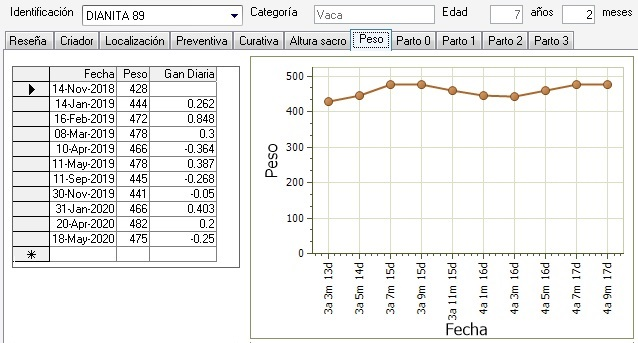
\includegraphics[scale=0.92]{img/ejpesos.jpg}
	 \end{center}
	 \caption{Ejemplo de seguimiento digital de peso en la res ``Dianita''. \label{ejpesos}}
\end{figure}

Los datos almacenados en este software, muestran registros de peso bimensual o trimestral, genealogía, suministro de medicamentos y producciones lecheras semanales.
No obstante, aún cuando este software ofrece una gran ventaja para el seguimiento de los datos, se encuentra limitado a las pocas licencias ofrecidas para su manejo. Por lo tanto es plausible considerar alternativas para el análisis, seguimiento de datos y toma de decisiones futuras, lo que justifica nuevamente la realización de este proyecto.